\documentclass[a4paper,10pt,spanish,oneside]{article}

% Preámbulo - Parte A

\usepackage[utf8]{inputenc} % Soporte para los acentos
\usepackage[T1]{fontenc}

\usepackage[spanish]{babel} % Capítulos, seciones, etc. en español

\usepackage[margin=2cm]{geometry} % Diseño del documento

\usepackage{multicol} % Escribir doble columna

\usepackage{xcolor} % Usar colores
\usepackage{pstricks}

\usepackage{enumerate} % Cambiar etiquetas de numeración
\usepackage[shortlabels]{enumitem} % Manejo adicional de etiquetas de numeración

\usepackage{graphicx} % Manejo de gráficos y figuras

\usepackage{makeidx} % Índice alfabético

% Paquetes adicionales de símbolos matemáticos
\usepackage{amsmath,amssymb,amsfonts,latexsym,cancel} 

% \usepackage{pslatex} % Fuente Times
% \usepackage{mathpazo} % Fuente Palatino
% \usepackage{mathptmx} % Fuente Times
% \usepackage{bookman} % Fuente Bookman
\usepackage{newcent} % Fuente New Century Schoolbook
% \usepackage{helvet} % Fuente Helvetica
% \usepackage{palatino} % Fuente Palatino
% \usepackage{pxfonts} % Fuente 
% \usepackage{txfonts} % Fuente
% \usepackage{concrete} % Fuente
% \usepackage{cmbright} % Fuente
% \usepackage{fourier} % Fuente

\usepackage{booktabs} % Opciones adicionales para el entorno tabular
\usepackage{longtable} % Para tablas de más de una página

\usepackage{tikz} % Creación de gráficos

% \usepackage{titlesec} % Personalizar capítulos y secciones

% Preámbulo - Parte B

\pagestyle{headings}

%\pagestyle{myheadings} % Numeración de página en la parte superior

\usepackage{titlesec}

\titleformat{\section} % command
			[display] % shape
			{\usefont{T1}{phv}{b}{n}\LARGE} % format
			{} % label
			{1pt} % sep
			{\thesection.\hspace{0.5em}} % before code
			
\titleformat{\subsection} % command
			[display] % shape
			{\usefont{T1}{phv}{b}{n}\Large} % format
			{} % label
			{1pt} % sep
			{\thesubsection.\hspace{0.5em}} % before code
			
\titleformat{\subsubsection} % command
			[display] % shape
			{\usefont{T1}{phv}{b}{n}\large} % format, fuentes: lmss,pag,phv
			{} % label
			{1pt} % sep
			{\thesubsubsection.\hspace{0.5em}} % before code		

\titleformat{name=\section,numberless}
			[display]
			{\usefont{T1}{phv}{b}{n}\LARGE}
			{}
  			{1pt}
  			{}
			\titlespacing*{\section}{0pt}{1pt}{1pt}

\title{\Huge\usefont{T1}{lmss}{b}{n} Procesamiento Digital de Señales\\
Parcial 2}
\author{Gianfranco Fagioli, Gaspar Oberti, Franco Matzkin, Facundo Salmerón, \\
		Darién Julián Ramírez, Iván Schweikofski y \textit{el Creador de la Bíblia}. 						\vspace{1em}\\ 
		\textbf{\textit{Distribúyase y mejórese.}}}
\date{\vspace{-5ex}}

\begin{document}

\maketitle %Crea la página de título

\tableofcontents

\newpage

\section{Diseño de filtros digitales}

\subsection{¿Qué diferencias y similitudes existen entre los conceptos de sistema y filtro?}

\begin{enumerate}[1.]
\item Ambos relacionan la entrada y la salida mediante:

	\begin{itemize}
	\item Una ecuación (digitales).
	\item Hardware (analógicos).
	\end{itemize}
	
\item Los filtros son un caso particular de sistema LTI (no introducen componentes frecuenciales).

\item Los filtros son un sistema pero se estudian desde la perspectiva de \textit{¿qué se quiere dejar pasar o qué no?}.

\begin{align*}
\textit{Filtro}\implies\textit{Sistema}
\end{align*}

\end{enumerate}

\vspace{1em}

\subsection{Explique que es un filtro de compensación de fase, un filtro de fase lineal y un filtro adaptativo.}

\begin{itemize}
\item Clasificación de filtros según su comportamiento en el tiempo:

\begin{itemize}
\item \textit{Filtro adaptativo:} Se adaptan al contexto variando en el tiempo los 				parámetros característicos (ancho de banda, frecuencia de corte, etc). El hecho de 				tener coeficientes variables del filtro, es necesario cuando se conocen \textit{a 				priori} las características estadísticas de la señal a filtrar o cuando se conoce y se 		sabe que son variables en el tiempo.\\
Se usan para analizar señales aleatorias no estacionarias.
\end{itemize}
		
\item Clasificación de filtros según su fase:
	
\begin{itemize}
\item \textit{Filtro de fase lineal:} Modifican la fase de la señal de entrada 		de forma lineal, proporcional a la frecuencia, independiente del módulo.
		
\item \textit{Filtro de compensación de fase:} No eliminan componentes frecuenciales, sólo modifican la fase. Tienen como finalidad compensar problemas de distorción de fase que sean previos a la aplicación del filtro.
\end{itemize}				
		
\end{itemize}

\subsection{Ejemplifique dos casos de aplicación donde se requiera la utilización de filtrado estático y adaptativo respectivamente. Justifique su respuesta.}

\begin{enumerate}[a.]

\item \textit{Filtro estático:} Siempre funcionan filtrando de la misma manera, osea es LTI (Lineal e Invariante en el Tiempo).

\begin{itemize}
\item \textit{Ejemplo:} un ECG que se transmite por radio frecuencia el cuál se sabe que va a poseer ruido desde la frecuencia 50Hz hasta 80Hz \textit{siempre}, entonces aplico un filtro estático rechaza-banda para eliminar la misma.

\item \textit{Ejemplo:} filtro analógico implementado electrónicamente para eliminar algunas componentes de ruido conocidas (rechaza banda) en la señal del monitor

\item \textit{Ejemplo:} se puede aplicar un filtro a una señal de conversación entre un adulto y un niño para eliminar la voz del adulto por ejemplo utilizando un filtro pasa bajo.
\end{itemize}

\item \textit{Filtro adaptativo:} Se adaptan al contexto variando en el tiempo los 				parámetros característicos, osea es LTV (Lineal y Variante en el Tiempo). El hecho de tener coeficientes variables del filtro, es necesario cuando se conocen \textit{a priori} las características estadísticas de la señal a filtrar o cuando se conoce y se sabe que son variables en el tiempo.\\
Se usan para analizar señales aleatorias no estacionarias.

\begin{itemize}
\item \textit{Ejemplo:} Cualquier sistema en el que las características del ruido no sean constantes, ya sea un ECG que va variando su ruido o un celular el cuál posee dos micrófonos, uno para tomar la voz y otro para tomar el ruido, las cuales son aleatorias y van cambiando en el tiempo, entonces el filtro adaptativo tiene que tomar ambas y a la señal de la voz restarle el ruido interpretado por el otro micrófono. 

\item \textit{Ejemplo:} La transmisión de un fax donde la misma puede haber perturbaciones en la señal eléctrica en el envío, entonces se coloca un filtro adaptativo para compensar estas perturbaciones que puede haber en la transmición.

\item \textit{Ejemplo:} Cuando se realiza un análisis de electrocardiograma la señal de la actividad eléctrica del corazón se ve afectada por la interferencia de la fuente eléctrica del aparato medidor. Una forma de eliminar correctamente este ruido es obtener la señal de la fuente y hacer variar los coeficientes del filtro según la frecuencia que tenga la señal de la fuente.

\item \textit{Ejemplo:} Cancelación de eco de una señal de voz mediante filtro adaptativo. Por ejemplo, en la comunicación telefónica cuando se utiliza altavoz, la señal producida por el parlante se introduce en el micrófono. Se utiliza un filtro adaptativo para limpiar la señal de micrófono haciendo variar los coeficientes del filtro según las frecuencias que tenga la señal de voz.
\end{itemize} 

\end{enumerate}

\subsection{Liste las ventajas y desventajas de utilizar un filtro de Butterworth.}

\begin{enumerate}[(+)]
\item No posee distorciones en la banda de paso ni en la de rechazo.
\end{enumerate}

\begin{enumerate}[(-)]
\item La banda de transición es más grande que para los otros filtros a un mismo grado.
\end{enumerate}

\subsection{Liste las ventajas y desventajas de utilizar un filtro de Chebyshev tipo II.}

\begin{enumerate}[(+)]
\item Posee una banda de transición más angosta con respecto a Butterworth.
\item Se puede escoger su paridad para la banda de rechazo.
\item Al aumentar su orden, se estrecha la banda de transición.
\end{enumerate}

\begin{enumerate}[(-)]
\item Ya tiene definida su fase y no se puede controlar, es decir, no se puede llegar a una
fase lineal a diferencia de los FIR (\textit{Finite Impulse Response}).
\item Puede llegar a ser inestable por ser un filtro recursivo.
\item Se requiere una gran presición numérica para evitar la inestabilidad.
\item Posee ondulaciones en la banda de rechazo.
\item Banda de paso monótonamente decreciente.
\end{enumerate}

\begin{itemize}
\item Los filtros Chebyshev de tipo II difieren de los de tipo I en que en vez de presentar ondulaciones en la banda de paso, éstas se encuentran en la banda de rechazo (siempre respetando un margen de error determinado). Por lo tanto, en la banda de paso la señal pasará sin sufrir alteraciones en la magnitud. Dependiendo del problema en particular, éstas oscilaciones pueden importar en mayor o menor medida.

\item Respecto al filtro de Butterworth, posee como ventaja que la banda de transición es más estrecha, pero como desventaja las oscilaciones en la banda de rechazo.

\item Respecto al elíptico, la ventaja es que posee menos oscilaciones pero como desventaja posee una banda de transición mayor.
\end{itemize}

\subsection{Detalle los pasos para el diseño de un filtro de Chebyshev tipo II a partir de su prototipo analógico.}

\begin{enumerate}[1.]
\item Se realiza en diseño analógico del filtro pasa bajo normalizado en el plano $s$, se establece el orden del filtro según los requerimientos.

\item \textit{Tranformación en frecuencia:} se convierte en filtro pasa bajo, pasa banda o rechaza banda y escalar para cambiar la frecuencia de corte.

\item \textit{Tranformación conforme:} se pasa al dominio digital, es decir, del dominio $s$ al dominio $z$. Se puede hacer con una transformación bilineal.
\end{enumerate}

Los pasos $2$ y $3$ se pueden intercambiar.

\subsection{Describa sucintamente una técnica de diseño de filtros IIR y una de filtros FIR.}

\begin{enumerate}[a.]
\item \textit{Técnica de diseño de filtros IIR}

\begin{enumerate}[1)]
\item \textbf{Especificación} de las características de la señal (tipo de fuente de la señal, frecuencia de muestreo, ancho de banda de la señal) y la respuesta en frecuencia y tolerancia (atenuación de la banda de paso, atenueación en la banda de rechazo, frecuencia de paso, frecuencia de rechazo, frecuencia de corte).

\item Seleccionar uno de los métodos para calcular los \textbf{coeficientes} $a_{k}$ y $b_{k}$ de un filtro IIR.

\begin{itemize}
\item \textit{Método 1:} 

\begin{itemize}
\item Diseño analógico (filtro pasa bajo normalizado).
\item Tranformación en frecuencia (analógica, en $s$).
\item Transformación conforme (bilineal).
\end{itemize}

\item \textit{Método 2:}

\begin{itemize}
\item Diseño analógico (filtro pasa bajo normalizado).
\item Transformación conforme (bilineal).
\item Tranformación en frecuencia (digital, en $z$).
\end{itemize}

\item \textit{Método directo:}

\begin{itemize}
\item Colocación de polos y ceros.
\end{itemize}

\end{itemize}

\item \textbf{Realización}, donde se convierte la función de transferencia en una estructura de filtro adecuada.

\item Se analizan los \textbf{errores} de cuantización, redondeo, número de bits, etc.

\item \textbf{Implementación} del filtro en \textit{software} o \textit{hardware}.

\end{enumerate}

\item \textit{Técnica de diseño de filtros FIR (Método de Fourier y Ventaneo)} 

\begin{enumerate}[1)]
\item \textbf{Especificación de requerimientos}, módulo y fase de la respuesta en frecuencia.

\item \textbf{Muestreo} de la respuesta en frecuencia.

\item Pasaje al dominio temporal mediante la TDF inversa. No causal y de duración infinita (\textit{sinc}).

\item Truncado temporal con ventanas teniendo en cuenta el efecto de Gibbs (relación entre el lóbulo central y los lóbulos laterales).

\item Corrección de amplitud multiplicando la señal por un valor que la aumenta o la disminuye.

\item Se causal el filtro realizando un corrimiento de la señal.
\end{enumerate} 

\end{enumerate}

\subsection{Apéndice}

\subsubsection{Comparativa de filtros}

Para un mismo orden:\\

\resizebox{\linewidth}{!}{
\begin{tabular}{lcccc} \toprule 
& Butterworth & Chebyshev Tipo 1 & Chebyshev Tipo 2 & Elíptico \\ \midrule
Banda de transición & Grande & Media & Media & Chica \\
Ondulaciones & No posee & Banda de paso & Banda de rechazo & Bandas de paso y rechazo \\
Para orden par-impar & - & Formas diferentes & Formas diferentes & Formas diferentes \\
Monotonía decreciente & En todas las bandas & Banda de rechazo & Banda de paso & No posee \\ \bottomrule
\end{tabular}
}

\section{Identificación de Sistemas}

\subsection{Escriba una definición de identificación de sistemas.}	

Proceso mediante el cual se pueden determinar la estructura y parámetros característicos de un sistema cuyas características intrínsecas se desconocen. En algunos casos la estructura del sistema puede ser conocida o supuesta \textit{a priori} y la identificación se reduce a la búsqueda de los parámetros.

\subsection{¿Cuáles son las limitaciones del método de predicción lineal?}

\begin{enumerate}[1.]
\item Supone que el sistema es lineal.
\item Sirve sólo para determinar los coeficientes del sistema (no el orden).
\item Para que produzca una buena estimación se necesita un orden muy alto.
\item La ecuación de tranferencia posee sólo polos.
\end{enumerate}

\subsection{Indique si las siguientes afirmaciones respecto a los métodos de identificación de sistemas basados en predicción lineal son correctas o no, justificando sus respuestas:}

\subsubsection{No pueden utilizarse en sistemas con entradas aleatorias.}

\textit{Falso.} \\

Para señales aleatorias estacionarias también se cumple $\mathbf{Ra}=-\mathbf{r}$. \\

Para señales aleatorias no estacionarias sólo funciona para procesos localmente estacionarios que pueden ser fragmentados en procesos estacionarios.

\subsubsection{Son los métodos más sencillos para identificar un sistema lineal de orden 		pequeño.}	

\textit{Falso.} \\

Existen métodos que permiten estimar fácilmente los parámetros característicos de sistemas lineales de orden 3 o menor. Consisten en estimular al sistema con un \textit{delta de Dirac} o el escalón y estudiar la respuesta temporal.

Mediante Laplace se puede escribir

\begin{align*}
Y(s) &= H(s)X(s)
\end{align*}

$y$ es la respuesta, $x$ es la entrada y $H$ la transferencia.

$X(s)$ del \textit{delta de Dirac} es 1, $Y(s)=H(s)$ donde haciendo la transformada inversa de la salida obtenemos la transferencia del sistema.

Otra forma es estimular el sistema con senoidales de frecuencia variable en el rango de interés y analizar la respuesta en frecuencia de la salida.

\subsubsection{No sirven para encontrar los parámetros de un sistema ARMA.}

\textit{Falso.}\\

Cualquier sistema ARMA puede ser aproximado mediante un sistema AR a través de

\begin{align*}
H(z) &= G\frac{B(z)}{A(z)}\approx\frac{G}{C(z)}
\end{align*}

$C(z)$ es de orden infinito pero se puede aproximar el sistema ARMA haciendo $C(z)$ del mismo orden  que $A(z)$

\begin{align*}
H(z) &= \frac{G}{1+\sum_{k=1}^{p}a_{k}z^{-k}}
\end{align*}

quedando la ecuación de recurrencia

\begin{align*}
s_{n} &= \sum_{k=1}^{p}a_{k}s_{n-k}+G\mu_{n}
\end{align*}

\begin{quote}
$p$: orden óptimo.\\
$G$: Ganancia.\\
$\mu_{n}$: entrada en el instante $n$.\\
\end{quote}

\subsubsection{Pueden extenderse fácilmente a los sistemas no lineales.}

\textit{Falso.}\\

Eliminar el supuesto de linealidad implica costos computacionales altos en sus implementaciones. Éstas técnicas no convencionales pueden utilizar algoritmos genéticos, redes neuronales, programación dinámica, búsqueda aleatorias y otras.

\subsection{Deduzca la ecuación de Wiener-Hopf utilizada en el método de predicción lineal para el caso de señales determinísticas.}

Sea $s_{n}$ la salida del sistema para el instante $n$, se aproxima el sistema mediante

\begin{align*}
\hat{s}_{n} &= -\sum_{k=1}^{p}a_{k}s_{n-k}
\end{align*}

donde $p$ es el orden óptimo de aproximación y $a$ los coeficientes del sistema.\\

El error cuadrático de esta aproximación para la $n$-ésima muestra está dado por

\begin{align*}
e_{n}^{2} &= (s_{n}-\hat{s}_{n})^{2}=(s_{n}+\mathbf{a}^{T}\mathbf{s_{n}})^{2}
\end{align*}

\begin{align*}
e^{2} &= \sum_{n}(s_{n}+\mathbf{a}^{T}\mathbf{s_{n}})^{2}
=\sum_{n}(s_{n}^{2}+2\mathbf{a}^{T}s_{n}\mathbf{s_{n}}
+\mathbf{a}^{T}\mathbf{s_{n}}\mathbf{s_{n}}^{T}\mathbf{a})
\end{align*}

Se quiere minimizar este error optimizando los coeficientes del sistema, por lo tanto se calcula el gradiente

\begin{align*}
\nabla_{a}e^{2} &= 0 \\
\nabla_{a}e^{2} &= \sum_{n}2s_{n}\mathbf{s_{n}}
+2\left(\sum_{n}\mathbf{s_{n}}\mathbf{s_{n}}^{T}\right)a=0 \\
\left(\sum_{n}\mathbf{s_{n}}\mathbf{s_{n}}^{T}\right)a &= -\sum_{n}s_{n}\mathbf{s_{n}} \\
(\textit{Matriz de correlación})a &= -\textit{Vector de correlación} \\
\mathbf{R}a &= -\mathbf{r}
\end{align*}

Esto conforma un sistema de ecuaciones lineales denominado \textit{sistema de Wiener-Hopf}.

\subsection{Deduzca la ecuación para el cálculo de la ganancia en el método de predicción lineal.}

Sea $s_{n}$ la salida del sistema en el tiempo $n$ y $\hat{s}_{n}$ la estimación del sistema AR dada por

\begin{align*}
\hat{s}_{n} &= -\sum_{k=1}^{p}a_{k}s_{n-k} & p &= \textit{orden del sistema}
\end{align*}

el error se puede ver como

\begin{align*}
e_{n} &= s_{n}-\hat{s}_{n}=G\mu_{n} 
\end{align*}

Se debe asegurar que la energía total de la señal de entrada sea igual a la energía total de la señal del error.

Las entradas que interesan son la entrada impulsiva y la de ruido blanco. Para entrada impulsiva

\begin{align*}
h_{n} &= -\sum_{k=1}^{n}a_{k}h_{n-k}+G\delta_{n}
\end{align*}

A partir del sistema de Wiener-Hopf

\begin{align*}
\mathbf{R}\mathbf{a} &= -\mathbf{r}
\end{align*}

se puede escribir

\begin{align*}
\mathbf{r}^{T}\mathbf{a} &= -r_{0}+G^{2} \\
G^{2} &= \mathbf{r}^{T}\mathbf{a}+r_{0}=E_{p}
\end{align*}

Para el ruido blanco es la misma expresión.

\subsection{Describa los métodos de estimación de orden y liste sus ventajas relativas.}

\begin{enumerate}[1.]
\item \textit{Error de predicción final:}

Utiliza la medición de los errores residuales en la resolución de los \textit{sistema de Wiener-Hopf}. Se asume una entrada no correlacionada y con espectro plano.

El mínimo error promedio para el sistema de orden $p$ está dado por

\begin{align*}
E_{p} &= r_{0}+\mathbf{r}^{T}\mathbf{a}
\end{align*}

Error normalizado

\begin{align*}
V_{p} &= \frac{E_{p}}{r_{0}}
\end{align*}

$V_{p}$ es monótono decreciente con $p$ y acotado.

Como se utilizan secuencias infinitas, la pendiente $V_{p}$ no se hace exactamente cero. Por eso se utiliza un umbral para la tolerancia.

\begin{align*}
1-\frac{V_{p+1}}{V_{p}} &< \gamma & \textit{(-) El orden obtenido es subjetivo} \\
&& \textit{(+) Es fácil de calcular}
\end{align*}

El incremento de orden se detiene cuando se cumple la inecuación.

\item \textit{Criterio de Akaike:}

Para el problema de todos polos y asumiendo una distribución gaussiana en la señal, se mide el error según

\begin{align*}
I_{p} &= \log{E_{p}}+\frac{2p}{N_{e}} & \textit{El orden es único}
\end{align*}

No es el número efectivo de la muestra de la señal, es decir, contemplando los efectos del ventaneo de la señal. Se calcula mediante la relación de la energía de la ventana utilizada y la energía de la ventana cuadrada.

\end{enumerate}

En el error de predicción final, a partir de cierto orden su amplitud relativa se mantiene constante a diferencia del método de Akaike el cual posee un mínimo en el orden óptimo. Akaike permite detectar más fácilmente el orden óptimo.

\section{Procesamiento de la Voz}

\subsection{Describa y clasifique desde el punto de vista fenomenológico a la señal producida a nivel de las cuerdas vocales. ¿Qué características posee su espectro? Grafique.}

Fenomenológicamente la señal es estacionaria por tramos y cuasi-periódica, ventanas de 10 a 30 milisegundos.

Su espectro es un tren de pulsos espaciados $F_{0}$ que es la frecuencia fundamental la cual posee información del hablante y de la entonación.\\

\begin{minipage}{0.5\linewidth}

\begin{center}
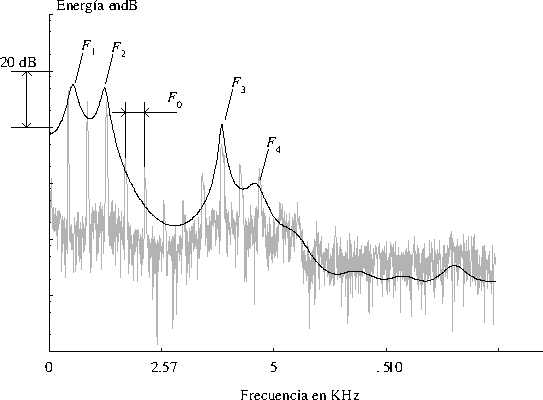
\includegraphics[width=\linewidth]{p2voz3}
\end{center}

\end{minipage} \hfill \begin{minipage}{0.5\linewidth}

\begin{center}
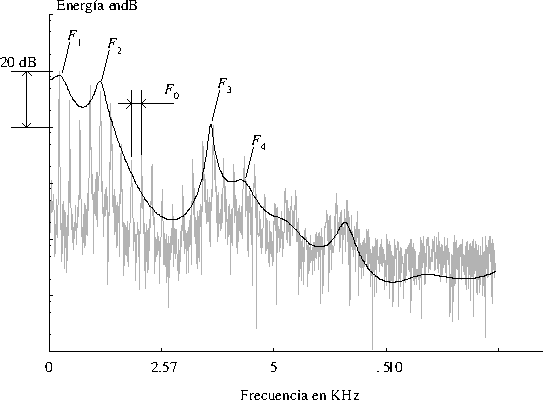
\includegraphics[width=\linewidth]{p2voz4}
\end{center}

\end{minipage}

\subsection{La figura representa el modelo lineal de producción de la señal de voz:}

\subsubsection{¿Qué tipos de señales de excitación se utilizan? ¿Qué parámetros definen 			cada tipo de excitación? ¿Cómo los estimarías?}
	
La señal de excitación corresponde al impulso glótico del tracto vocal. Éste posee una frecuencia $F_{0}$ denominada frecuencia fundamental.\\

El parámetro que define ésta excitación es la frecuencia fundamental $F_{0}$.\\

Se puede estimar mediante:

\begin{enumerate}[1.]
\item Analizando los cuasi-períodos de la señal en el dominio temporal (restando dos picos y viendo la frecuencia de muestreo).

\item \textit{Autocorrelación sin sesgo:} se calculan los coeficientes de autocorrelación $\displaystyle y[k]=\sum_{n}x[n]x[n-k]$.

\item Analizando el ceptrum real de la señal y observando el tiempo donde aparece el segundo pico.

\item \textit{Clipping:} eliminar información de la parte central de la señal que no es necesaria para hallar $F_{0}$.

\item \textit{Autocorrelación pesada:} se hace \textit{autocorrelación sin sesgo} y \textit{clipping}, suavizar la estimación del tiempo para cada cuasi-período según $AP[\tau,q]$
\end{enumerate}
	
\subsubsection{¿Qué modela el bloque denominado \textit{sistema} y de que tipo es? ¿Cuántos 	parámetros se necesitan definirlo? ¿Cómo se estiman estos parámetros?}

\begin{center}
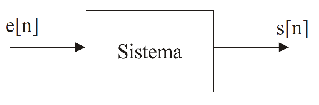
\includegraphics{p2voz2}
\end{center}

El sistema es la función de transferencia del tracto vocal.\\

Se define con las frecuencias formantes que pueden variar con el tiempo para producir los diferentes fonemas.\\

Éstas se pueden estimar hallando los máximos de la función de transferencia que se hubican después del primer máximo. La función de tranferencia se halla calculando el ceptrum $IFFT(\log|IFFT(x[n])|)$ y tomando los 13 primeros coeficientes.

\subsection{Proponga un método para calcular la frecuencia fundamental ($F_{0}$) de un tramo de señal de voz.}

\begin{enumerate}[1.]
\item Analizando los cuasi-períodos de la señal en el dominio temporal (restando dos picos y viendo la frecuencia de muestreo).

\item \textit{Autocorrelación sin sesgo:} se calculan los coeficientes de autocorrelación $\displaystyle y[k]=\sum_{n}x[n]x[n-k]$.

\item Analizando el ceptrum real de la señal y observando el tiempo donde aparece el segundo pico.

\item \textit{Clipping:} eliminar información de la parte central de la señal que no es necesaria para hallar $F_{0}$.

\item \textit{Autocorrelación pesada:} se hace \textit{autocorrelación sin sesgo} y \textit{clipping}, suavizar la estimación del tiempo para cada cuasi-período según $AP[\tau,q]$
\end{enumerate}

\subsection{¿A que se denominan \textit{frecuencias formantes}? ¿Cómo se denotan y que importancia tienen en la generación de la voz?}

Las \textit{frecuencias formantes} son las frecuencias en las que se encuentran máximos locales en el dominio frecuencial de la respuesta al impulso del tracto vocal. El \textit{primer} $(F_{1})$ y el \textit{segundo} $(F_{2})$ pico son frecuencias que permiten identificar el \textit{fonema sonoro} y \textit{los demás picos} $(F_{3},F_{4})$ permiten identificar la identidad del hablante.

Son picos de mayor intensidad en el espectro de sonido. Se producen por la resonancia del tracto vocal que modifica la amplitud de los armónicos del sonido. Frecuencias amplificadas por resonancia.

\subsection{¿Qué es la escala de mel y cómo se utiliza para el análisis de voz?}

La \textit{escala de mel} es una escala que relaciona la frecuencia percibida por el oido humano y la frecuencia física. Es decir, es una unidad de medida para la frecuencia percibida. Es no lineal ya que el oido es más sencible a los cambios de las frecuencias bajas que de las altas. Se determinó que $1000[mels]=1000[Hz]$.

\begin{align*}
F_{mel} &= 1000\log_{2}\left(1+\frac{f_{Hz}}{1000}\right)
\end{align*}

En el análisis de la voz, lo que se utiliza es un banco de filtros triangulares linealmente espaciados en la \textit{escala de mel}, que se le aplican a la señal en el dominio de las cuefrencias. Con esto se obtiene un vector de coeficientes de \textit{mel}. Una vez obtenidos se les aplica la transformada de coseno (más rápida que Fourier) obteniendo los coeficientes ceptrales en \textit{escala de mel} (CCEM) los cuales tienen información referida a la envolvente de los coeficientes de mel.

\subsection{Describa las hipótesis en las que se basa el análisis cepstral del habla para separar la señal de excitación, de la respuesta del tracto vocal ¿Son realistas estas hipótesis?}

La señal de excitación del tracto vocal y la respuesta del tracto vocal son independientes y varían de forma diferente, por lo que se pueden separar en el ceptrum.

La duración de la respuesta al impulso del sistema termina antes que el segundo pico del pulso de la señal de excitación.

la hipótesis inicial para poder realizar un análisis cepstral es que las componentes a evaluar tienen que distinguirse mucho en frecuencia, es decir, una tener frecuencia muy alta y la otra muy baja. Por eso funciona perfectamente para el análisis del habla.

La segunda hipótesis es que un ciclo de una las componentes tiene que terminar cuando empieza la otra, no se tienen que superponer.

\subsection{Considere la gráfica de una vocal sostenida $x[n]$ que se muestra en la Figura 1.(a). Indique, dibujando sobre la misma, un Período Fundamental ($T_{0}$) y estime (aproximadamente) su duración. La frecuencia de muestreo es de 8 kHz:}

El período es de $\displaystyle 60\left[\frac{muestras}{seg}\right]$ (observación).

\begin{align*}
T_{0} &= \frac{60[muestras]}{8000[Hz]}=7.5\times 10^{-3}[seg]
\end{align*}

\begin{minipage}{0.5\linewidth}

\subsubsection{Defina el \textit{cepstrum real} $c[n]$.}

\begin{align*}
c[n] &= \frac{1}{2\pi}\int_{-\pi}^{\pi}\log|x(e^{j\omega})|e^{j\omega}dw \\
&= IDFT(\log|DTFT(x[n])|)
\end{align*}

Tiene que ser complejo para poder reconstruir la señal.

\subsubsection{A partir de la Figura 1.(b), correspondiente al \textit{cepstrum real} del segmento de vocal mostrado en la Figura 1.(a), indique cómo estimar la Frecuencia Fundamental ($F_{0}$) del segmento y compare con el resultado obtenido en el punto anterior.}

\begin{align*}
F_{0} &= \frac{1}{T_{0}}=\frac{1}{7\times 10^{-3}[seg]}=142.85[Hz]
\end{align*}

\end{minipage} \hfill \begin{minipage}{0.5\linewidth}

\begin{center}
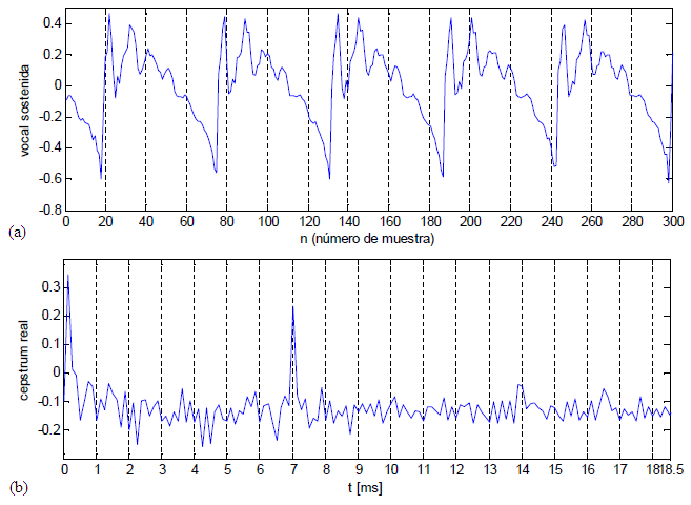
\includegraphics[width=\linewidth]{p2voz1}
\end{center}

\end{minipage}

\subsection{Proponga un método para contar la cantidad de cruces por cero de un tramo de señal de voz. ¿Cómo haría para que el método fuera robusto al ruido?}

La cantidad de cruces por cero nos da una estimación de la frecuencia de la señal. Se puede obtener verificando la cantidad de veces que la misma cambia de signo.

\begin{align*}
CPC &= \frac{1}{2}\sum_{n=1}^{N-1}(signo(x[n])-signo(x[n+1]))
\end{align*}

Es robusto al ruido ya que éste se le suma a la señal y no influye significativamente en la \textit{cantidad de cruces por cero}. Lo que puede ocurrir es que aumente un poco el número de los mismos cuando por ejemplo la señal pasa de positivo a negativo y cerca de ese instante el ruido oblique a la misma a subir y volver a bajar. Lo mismo puede ocurrir en el caso contrario pero a pesar de esto sigue siendo \textit{un buen estimador de la frecuencia de la señal}.

\subsection{Indique las consideraciones especiales que deben tenerse en cuenta al aplicar el método de predicción lineal a señales de voz. ¿En qué casos aplicaría el método adaptativo de Widrow?}

El \textit{método de predicción lineal} supone:

\begin{enumerate}[1.]
\item Un modelo AR (todos polos).

\item Un sistema lineal.

\item Una señal estacionaria o cuasi-estacionaria.
\end{enumerate}

Lo aplicaría cuando se quiere analizar una señal no estacionaria. En Widrow, el \textit{error cuadrático medio} (ECM) se aproxima mediante el \textit{error cuadrático instantáneo} (ECI):

\begin{align*}
\nabla\xi_{n}^{2} &= \frac{\partial e_{n}}{\partial a_{n}}
=\frac{\partial}{\partial a_{n}}(s_{n}+\mathbf{a_{n}^{T}}\mathbf{s_{n}})
\end{align*}

Remplazando en $a_{n+1}$.

\begin{align*}
a_{n+1} &= a_{n}-2\mu s_{n}\hat{s}_{n} & a_{n}\in[-0.5,0.5]
\end{align*}

$\mu$ determina la velocidad de convergencia.

\section{Análisis Tiempo-Frecuencia}

\subsection{Explique la necesidad de utilizar transformaciones tiempo-frecuencia.}

Estas tranformaciones son necesarias ya que la TDF no otorga información sobre los tiempos en los que ocurren las distintas fracuencias de la señal.

\subsection{Defina la \textit{Transformada de Fourier de Corta Duración} (STFT), en sus versiones continua y discreta.}

\begin{itemize}
\item \textit{Continua}

Dada una ventana real simétrica $g(t)=g(-t)$, se genera una base al desplazarla y modularla con una frecuencia $\xi$.

\begin{align*}
g_{u,\xi}(t) &= e^{i\xi t}g(t-u) & \textit{Átomo tiempo-frecuencia}
\end{align*}

Si $\|g_{u,\xi}(t)\|=1$ la STFT (\textit{Trandormada de Fourier de Tiempo Corto}) es

\begin{align*}
Sf(u,\xi) &= \int_{-\infty}^{\infty}f(t)g_{u,\xi}^{*}(t)dt
=\int_{-\infty}^{\infty}f(t)g(t-u)e^{-i\xi t}dt
\end{align*}

\item \textit{Discreta}

\begin{align*}
g_{m,l}[n] &= g[n-m]e^{\frac{-i2\pi ln}{N}} & \textit{Átomo tiempo-frecuencia} \\
Sf[m,l]=\langle f[n],g_{m,l}[n]\rangle &= \sum_{n=0}^{N-1}f[n]g[n-m]e^{\frac{-i2\pi ln}{N}}
\end{align*}

\end{itemize}

\subsection{Explique al menos dos maneras de interpretar conceptualmente a la STFT. Utilice gráficos detallando las magnitudes y unidades de los ejes.}

\begin{minipage}{0.3\linewidth}

\begin{enumerate}[1.]

\item Se puede interpretar como la \textit{Transformada de Fourier} aplicada al producto de una ventana por la función en cierto intervalo de tiempo.

\end{enumerate}

\end{minipage} \hfill \begin{minipage}{0.6\linewidth}

\begin{center}
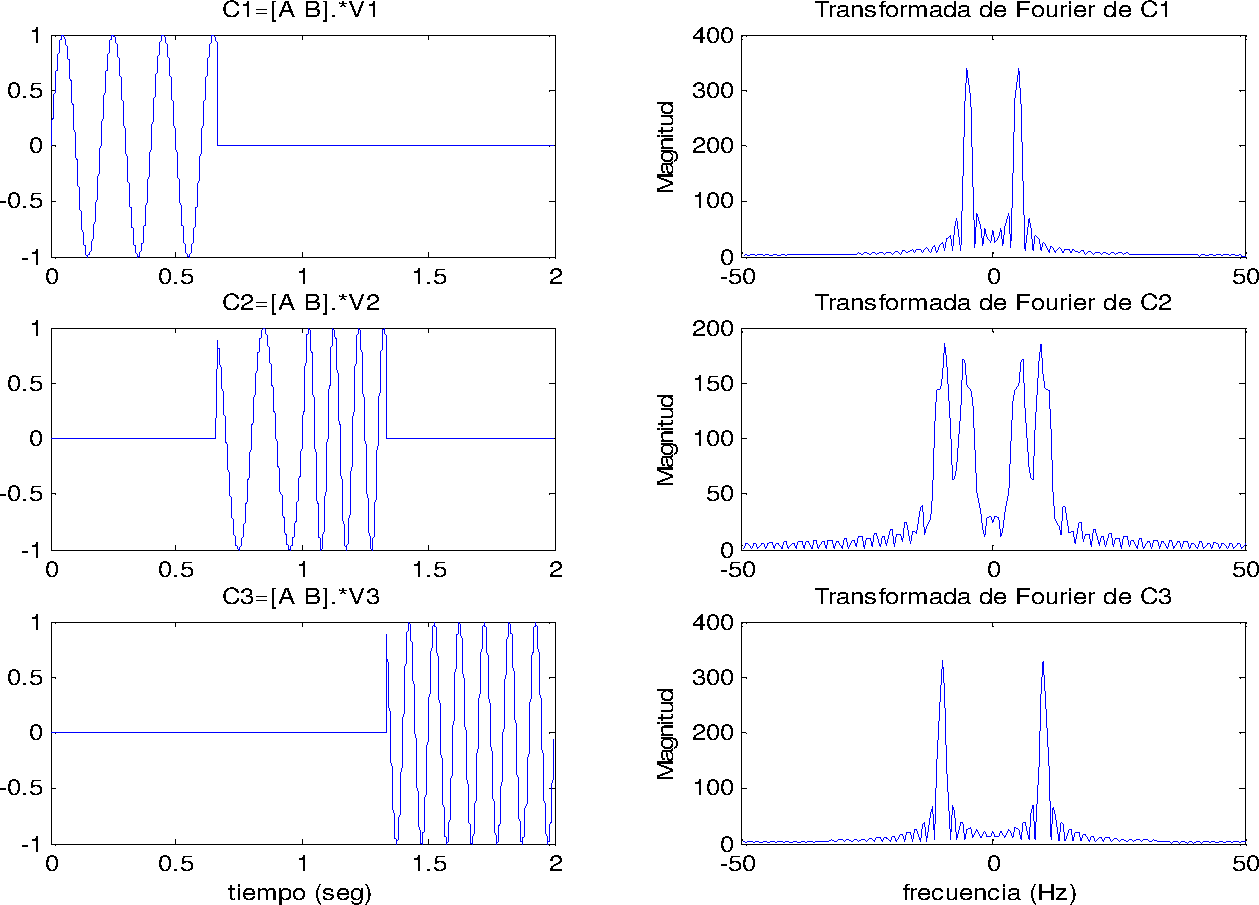
\includegraphics[width=\linewidth]{p2tf6}
\end{center}

\end{minipage} \\ \\

\begin{minipage}{0.3\linewidth}

\begin{enumerate}[2.]

\item Se puede representar mediante un espectrograma en el cual el eje de las absisas representa el tiempo y el de las ordenadas las frecuencias. En el interior se representa la energía de la transformada para cada instante de tiempo y en cada frecuencia.

\end{enumerate}

\end{minipage} \hfill \begin{minipage}{0.6\linewidth}

\begin{center}
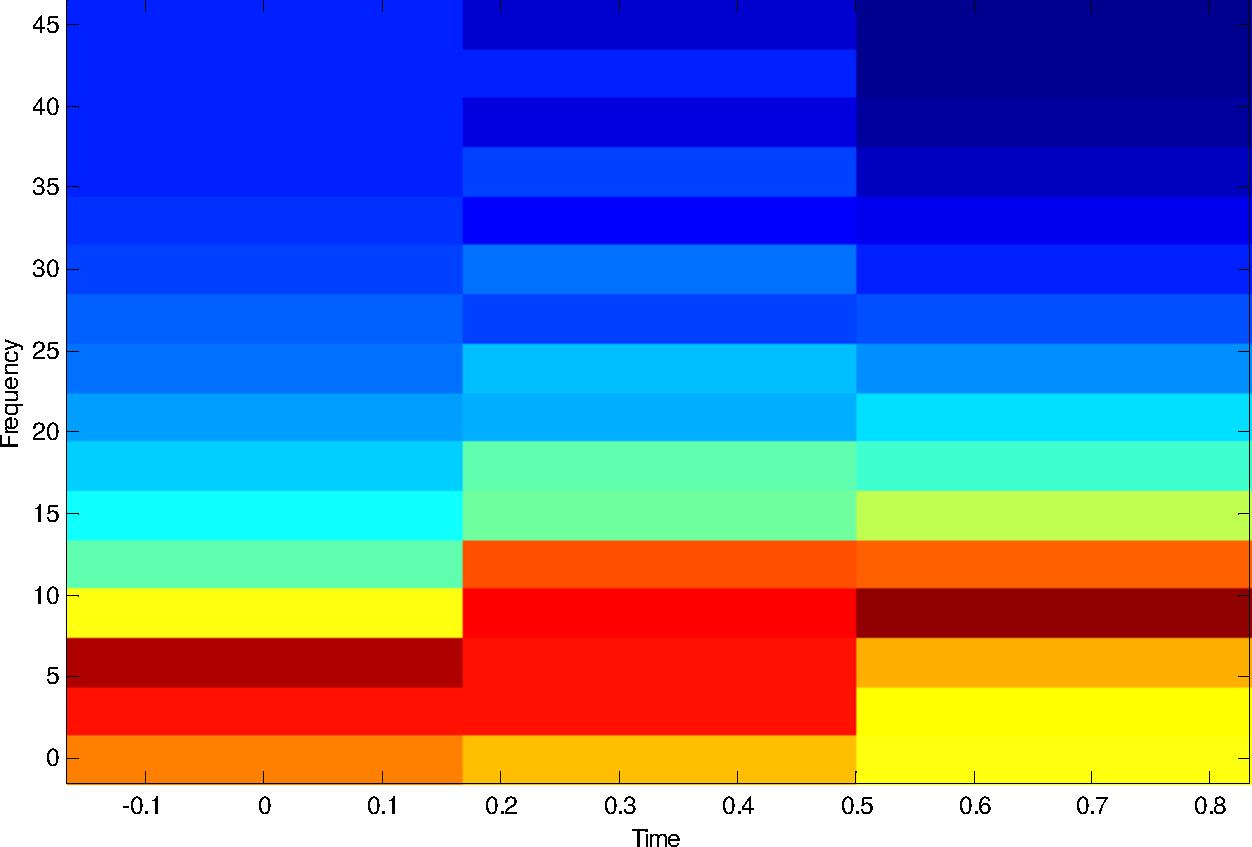
\includegraphics[width=\linewidth]{p2tf7}
\end{center}

\end{minipage}

\subsection{Explique en que consiste el \textit{principio de incertidumbre} y como se expresa analíticamente.} 

Consiste en que si se incrementa la resolución frecuencial disminuye la resolución temporal. Lo mismo ocurre para el caso contrario.

El principio de la incertidumbre de Heisenberg asegura que la varianza temporal $\sigma_{t}$ y la varianza frecuencial $\sigma_{\omega}$ de una función $f(t)\in L^{2}\mathbb{R}$ (espacio de Hilbert de dimensión infinita de señales de energía finita) satisfacen la siguiente inecuación:

\begin{align*}
\sigma_{t}\sigma_{\omega} &\geq \frac{1}{2}
\end{align*}

En la STFT, la función $g(t)$ permanece igual, sólo se desplaza en el tiempo por lo que la resolución es uniforme en tiempo y frecuencia.

\begin{align*}
\Delta t &= \textit{Tamaño de ventana}=T_{vent} \\
\Delta f &= \frac{1}{\Delta t}=\frac{1}{T_{vent}} \\
\implies\Delta_{t}\Delta_{f} &= 1
\end{align*}

\subsection{¿Es posible interpretar la STFT en términos de una \textit{base}? En caso afirmativo ejemplifique graficando algunos elementos de la misma.}

La STFT no es una base ya que para serlo debe ser un conjunto de vectores \textit{generador} y \textit{l.i}.

\begin{itemize}
\item Si las ventanas no se solapan pierdo información de la señal (no es \textit{generador}).

\item Si las ventanas se solapan hay información redundante (no es \textit{l.i.}).
\end{itemize}

El hecho de que la STFT no sea una base significa que no puedo reconstruir de manera exacta la señal original, ya que tendrá una combinación lineal de infinitas soluciones.


\subsection{Describa el algoritmo rápido para el cálculo de la Transformada Ondita Diádica.}

A la señal original se la filtra con un filtro \textit{pasa alto} $g$ y un \textit{pasa bajo} $h$ cuyas frecuencias de corte se establecen siempre a la mitad. Luego, con la salida de ambos se realiza un submuestreo (para cada salida de los filtros se descarta la mitad de las muestras). Lo que queda proveniente del filtro \textit{pasa alto} son los coeficientes de detalle de nivel 1.

A lo que salió del filtro \textit{pasa bajo} se le aplica el mismo procedimiento, aplicar $g$ y $h$, obtener los coeficientes de detalle nivel 2 y repetir hasta llegar a $a_{j}$.

Notar que como se está submuestreando, la frecuencia que puede tomar la señal se va reduciendo y los filtros cortan siempre por la mitad.

Cuando se llega a  $p_{i}$ se obtiene el coeficiente de detalle de nivel $p$ y el coeficiente de aproximación de nivel $p$.\\

Analíticamente:

\begin{align*}
a_{j+1}[p] &= \sum_{n=-\infty}^{\infty}h[n-2p]a_{j}[n] \\
d_{j+1}[p] &= \sum_{n=-\infty}^{\infty}g[n-2p]a_{j}[n]
\end{align*}

y para la resconstrucción:

\begin{align*}
a_{j}[p] &= \sum_{n=-\infty}^{\infty}h[p-2n]a_{j+1}[n]
+\sum_{n=-\infty}^{\infty}g[p-2n]d_{j+1}[n]
\end{align*}

\subsection{Defina la \textit{Distribución de Wigner-Ville} en su versión continua. Resuma ventajas y desventajas.}

Las STFT y las Wavelets calculan la correlación de la señal con familias de átomos tiempo-frecuencia, por lo que la resolución tiempo-frecuencia de éstas queda limitada a la resolución de sus átomos.

La distribución de Wigner-Ville presenta la densidad de energía en tiempo-frecuencia calculada mediante la correlación de la señal con ella misma desplazada en tiempo y frecuencia.

La aplicaciónde esta distribución es imitada debido a la existencia de términos de interferencia.

\begin{itemize}
\item \textit{Continua:}

\begin{align*}
P_{v}f(\mu,\xi) &= \int_{-\infty}^{\infty}f\left(\mu+\frac{\tau}{2}\right)
f^{*}\left(\mu-\frac{\tau}{2}\right)e^{-i\xi\tau}d\tau
\end{align*}

\item \textit{Discreta:}

\begin{align*}
P_{v}f[n,k] &= \sum_{p=-N}^{N-1}f\left[n+\frac{p}{2}\right]
f^{*}\left[n-\frac{p}{2}\right]e^{\frac{-i2\pi kp}{N}}
\end{align*}

$\displaystyle \frac{p}{2}$ son muestras intermedias, es necesario interpolar.\\

\end{itemize}

\textit{Ventaja:} Muy buena resolución frecuencial.\\

\textit{Desventaja:} Al ser una transformación cuadrática en $f$, aparecen términos que provocan interferencia.

\begin{align*}
P_{v}f &= P_{v}f_{1}+P_{v}f_{2}{\red +P_{v}[f_{1},f_{2}]+P_{v}[f_{2},f_{1}]}
& {\red \textit{términos de interferencia}}
\end{align*}

Tiene interferencias cruzadas entre $f_{1}$ y $f_{2}$, y ambas interferencias entre las frecuencias positivas y negativas de una misma $f$.

\subsection{Esquematice y compare las particiones del plano tiempo-frecuencia que se obtienen mediante una representación que utilice una base de \textit{deltas de Dirac}, la base de la \textit{Transformada Discreta de Fourier}, la \textit{Transformada de Fourier de Corta Duración} y la \textit{Transformada Onditas Discreta Diádica}.}

\begin{minipage}{0.5\linewidth}

\begin{enumerate}[1.]
\item \textit{Deltas de Dirac:}

\begin{center}
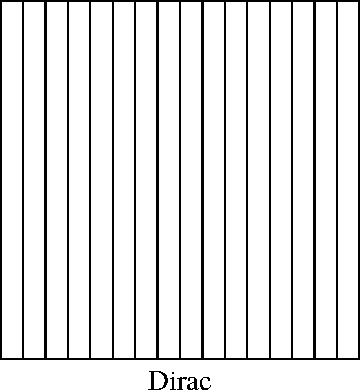
\includegraphics{p2tf1}
\end{center}

\end{enumerate}

\end{minipage} \hfill \begin{minipage}{0.5\linewidth}

\begin{enumerate}[2.]

\item \textit{Transformada Discreta de Fourier:}

\begin{center}
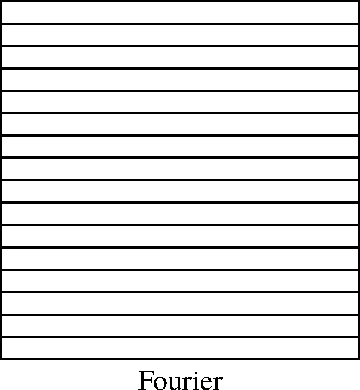
\includegraphics{p2tf2}
\end{center}

\end{enumerate}

\end{minipage}

\begin{enumerate}[3.]

\item \begin{center}
\textit{Transformada de Fourier de Tiempo Corto:}
\end{center}

\end{enumerate}

\begin{minipage}{0.5\linewidth}

\begin{center}
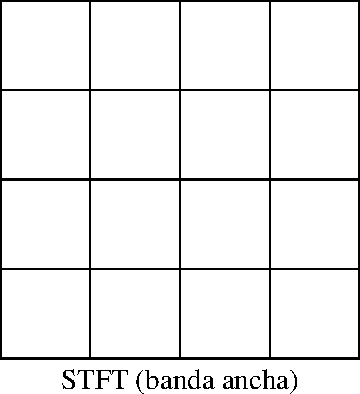
\includegraphics{p2tf3}
\end{center}

\end{minipage} \hfill \begin{minipage}{0.5\linewidth}

\begin{center}
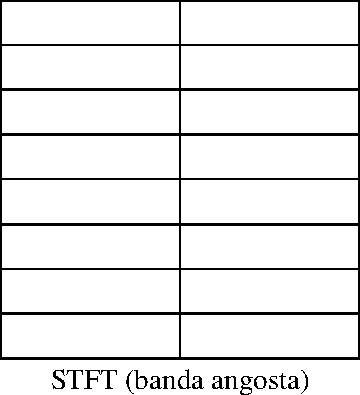
\includegraphics{p2tf4}
\end{center}

\end{minipage} \\

\begin{enumerate}
\item \textit{Transformada Onditas Discreta Diádica:}

\begin{center}
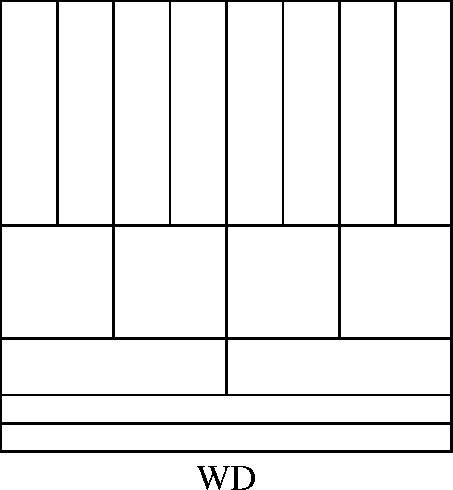
\includegraphics{p2tf5}
\end{center}

\end{enumerate}

\section{Problemas}

\subsection{Problema 1}
Se quieren enviar las fotos tomadas con la cámara de un celular por el canal de audio del mismo. Para ello se le requiere que escriba el algoritmo que permita transformar una imagen digital en una señal unidimensional real.

Tenga en cuenta las siguientes consideraciones:

	\begin{enumerate}[a.]
	\item La imagen se trataría como si fuera el espectrograma de la señal.
	\item La señal resultante deber ser audible en el rango 0-5 [KHz].
	\item Enumere y explique todos los pasos y parámetros necesarios.
	\end{enumerate}

\subsection{Problema 2}
Un grupo de ornitólogos está interesado en desarrollar un herramienta que les permita clasificar el canto de los pájaros a fin de monitorear en forma automática las poblaciones silvestres y sus variaciones debido a las corrientes migratorias. Se sabe que el canto de los pájaros está formado por sílabas y que éstas constituyen los
bloques de construcción elementales, en forma similar a como se da en el habla humana. En muchos tipos de canciones la mayoría de las sílabas pueden aproximarse como uno o varios pulsos sinusoidales breves que varían en amplitud y frecuencia. Sin embargo la variabilidad espectral de las canciones es varios ordenes de magnitud más rápida que en los humanos, requiriendo de una alta resolución temporal, del orden de 1 milisegundo. La energía espectral esta típicamente concentrada en una estrecha área entre 1 y 6 kHz, la cual varía para cada especie. Se le solicita diseñar una herramienta que permita extraer la información relevante de archivos de sonido
grabados adecuadamente, y detectar la especie a la cual corresponde, de entre las 14 especies en estudio.

\begin{figure}[!htbp]
\centerline{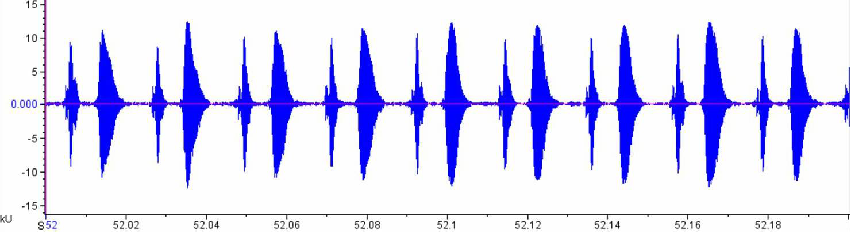
\includegraphics{p2preg1}}
\caption{Registro típico de la señal acústica del canto de un pájaro en función del tiempo (mins).}
\label{fig:p2preg1}
\end{figure}

\subsection{Problema 3}
Un grupo de biólogos marinos está interesado en desarrollar un herramienta que les permita clasificar el canto de las ballenas a fin de monitorear en forma automática las poblaciones salvajes y sus variaciones debido a las corrientes oceánicas. Se sabe que el canto está formado por sílabas y que éstas constituyen los bloques de construcción elementales, en forma similar a como se da en el habla humana. En muchos tipos de canciones la mayoría de las sílabas pueden aproximarse como uno o varios pulsos sinusoidales breves que varían en amplitud y frecuencia. Sin embargo, la variabilidad espectral de las canciones es varios ordenes de magnitud más rápida que
en los humanos, requiriendo de una alta resolución temporal, del orden de 1 milisegundo. La energía espectral esta típicamente concentrada en una estrecha área entre 1 y 6 kHz, la cual varía para cada especie. Se le solicita diseñar una herramienta que permita extraer la información relevante de archivos de sonido grabados adecuadamente, y detectar la especie a la cual corresponde, de entre las 14 especies en estudio.

\subsection{Problema 4}
A finales del siglo XX, un grupo de matemáticos israelíes propuso la existencia de un código secreto en la Biblia. El código fue \textit{descubierto} mediante una computadora en la versión hebrea del Antiguo Testamento (Torah), eliminando los espacios entre palabras, y convirtiendo el texto en una única palabra hebrea de 304.805 letras. Un programa exploraba esta larga tira en busca de las palabras y frases que se le ingresaban. El proceso comienza con la primera letra, primero de corrido, luego saltando de a una letra, luego de a dos, y así sucesivamente hasta
terminar. Seguidamente, se rehace el mismo proceso comenzando desde la segunda letra, y luego desde las demás hasta terminar. Se le solicita que proponga un algoritmo para el programa que realiza la búsqueda dentro del texto.

\subsection{Problema 5}
Se desea diseñar un sistema que permita convertir una imagen digital en una señal audible (en el rango de 0-4 kHz), para poderla transmitir por una linea telefónica analógica, de tal manera que posteriormente pueda reconstruirse nuevamente la imagen original. Proponga un algoritmo que permita realizar ambas tareas y realice
todas las consideraciones necesarias para su implementación.

\subsection{Problema 6}
En la sala del consejo directivo de la FICH se han realizado registros de voz mediante micrófonos ubicados frente a cada uno de los consejeros participantes y se quiere rescatar con mayor fidelidad la locución de uno de ellos en particular. Proponga un sistema que permita filtrar esta voz suponiendo que la señal registrada por todos los otros micrófonos puede ser considerada como el ruido de fondo que también se capta en el micrófono de interés.

\end{document}